

%%%%%%%%%%%%%%%%%%%%%%%%%%%%%%%%%%%%%%%%%%%%%%%%%%%%%%%%%%%%%%%%%%%%%%%%%%%%%%%%
\subsection{Architecture}

The footstep evaluation network is then used to feed the gait net
architecture shown in \autoref{fig:diagram-gaitnet-architecture}. The
gait net takes in the robot state information and ranked footstep
positions from the footstep evaluation network. It then outputs the
desired contact state\textemdash which feet should be in contact with
the ground. This information is then passed as constraints to the MPC.

\begin{figure}
  \centering
  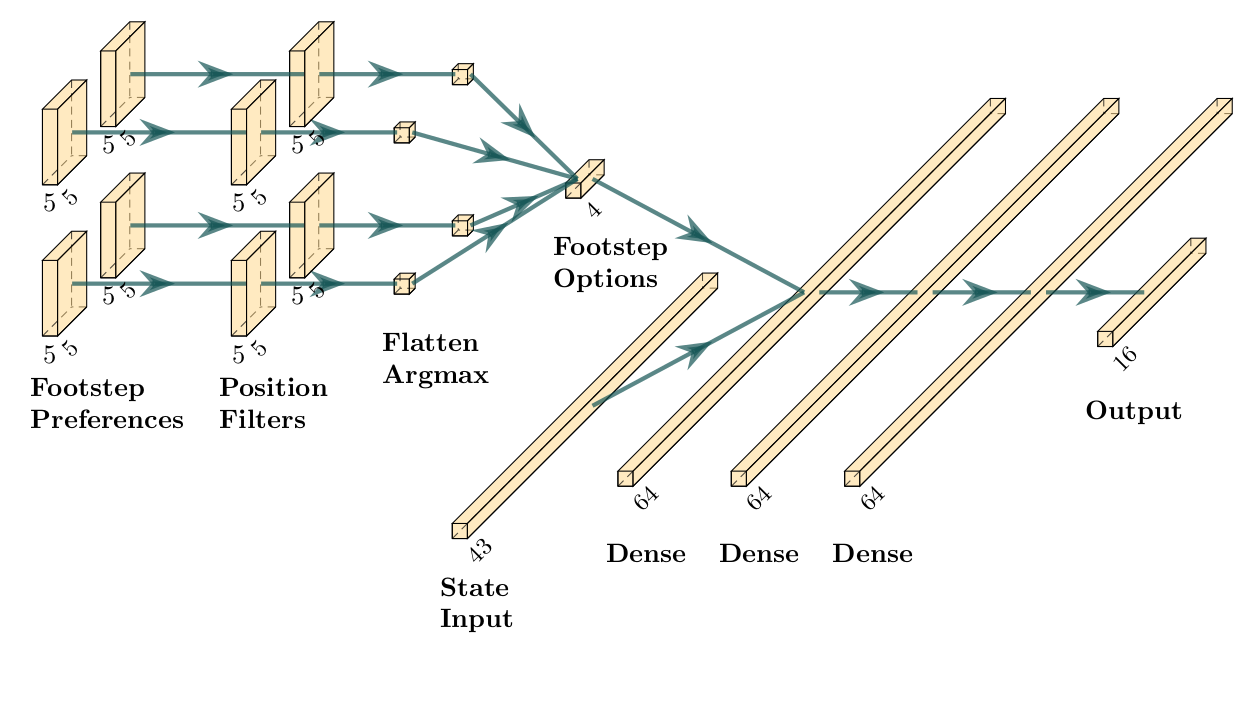
\includegraphics[width=0.75\linewidth]{images/diagrams/gait-network-architecture.png}
  \caption{Gait net architecture. Sections of the diagram include
    cost map pre-processing in yellow, footstep encoder in orange,
    state encoder in blue, and shared trunk in green. Cost maps for each
    foot are generated using ContactNet. The cost maps are then
    filtered based on the robot state and terrain data before being fed
    into the footstep encoder one at a time. The robot state is encoded
    before being combined with the footstep encodings in the shared
    trunk. The final output is the value of this option and the
  suggested swing duration.}
  \label{fig:diagram-gaitnet-architecture}
\end{figure}

%%%%%%%%%%%%%%%%%%%%%%%%%%%%%%%%%%%%%%%%%%%%%%%%%%%%%%%%%%%%%%%%%%%%%%%%%%%%%%%%
\subsection{Training}
